\documentclass[10pt]{article}
\usepackage{CJKutf8}
\usepackage[margin=1.2in]{geometry}

%\usepackage{algpseudocode}
%\usepackage{algorithm}

\usepackage{graphicx}
\usepackage{fmtcount}

\usepackage{multirow}

\usepackage[hyphens]{url}
\usepackage{hyperref}

\usepackage{array}
\usepackage{amsmath}
\usepackage{amssymb}

%\usepackage{natbib}

\usepackage{mathtools}

\usepackage{listings}
\usepackage{color}
\usepackage{booktabs}

% keywords: fixme

\sloppy

\begin{document}
\begin{CJK*}{UTF8}{gbsn}

\title{x64架构下{\tt C++}实现几种高效实用的位反转方法}

\author{Christian Knauth\\
柏林自由大学\\
信息学院
\and
Boran Adas\\
柏林自由大学\\
信息学院
\and
Daniel Whitfield\\
柏林自由大学\\
信息学院
\and
Xuesong Wang\\
柏林自由大学\\
信息学院
\and
Lydia Ickler\\
柏林自由大学\\
信息学院
\and
Tim Conrad\\
柏林自由大学\\
信息学院
\and
Oliver Serang\\
柏林自由大学\\
信息学院\\
\url{orserang@uw.edu}
}

\date{{\small \today}}

\maketitle

\begin{abstract}
\noindent 位反转是信号处理过程中的一个重要任务,同时它也是决定傅里叶变换效率的关键。
这篇文章将通过{\tt C++}实现现有的五种位反转计算方法:Stockham自动排序、朴素按位交
换、反转字节表查询交换、局部成对位交换以及高速缓存局部矩阵缓冲交换。 三种新的位反
转计算方法将会得到展示:使用归纳法的按位异或操作、闭型模板递归以及高速缓存参数无关的
模板递归法。第三种方法通过分解至更少位数的位反转和方阵转置实现。这些新的方法会通过理
论运行时间、实证编译时间以及实证运行时间与以上现有的五种方法进行比较。三种方法中最快
的相较于现有最快方法而言,极具优势;然而,最快的方法可以通过使用GPU的并行运算发掘更
多的潜力。
\end{abstract}

\section*{引言}
传统的Cooley-Tukey快速傅里叶变化(FFT)通过递归将问题转化为两个长度减半的FFT(
奇数项和偶数项)\cite{cooley:algorithm}。Cooley-Tukey方法在科学计算中极其重
要。它可以在$O(n \log(n))$步内计算两个长度为$n$的序列卷积,而非传统卷积计算所需
的$O(n^2)$步\cite{proakis:introduction}。Cooley-Tukey方法的简易、高效以及
通用性使它成为20世纪科学计算领域最具影响力的方法之一\cite{cipra:best}。

计算Cooley-Tukey FFT最简单的方法是非原位计算(out-of-place),并使用一个大小为$n$的buffer。
原数组中的数值可以被被复制到buffer中,于是原来数组中的偶数项现在占据着$0, 1, \ldots
\frac{n}{2}-1$的索引位置。同时,奇数项分布在$\frac{n}{2}, \frac{n}{2}+1, \ldots n-1$的位置上。这种使用buffer的方法一般被称为Stockham自动排序法。\cite{cochran:fast}



然而,计算一个原位(in-place) FFT(\emph{i.e.} 在不使用buffer的情况下,通过重写当前数组来
计算FFT)更具挑战性。通过Stockham FFT计算偶数项的变换与一个$\frac{n}{2} \times 2$
矩阵转置相当。列如一个长度$n=8$的数组索引是$[0, 1, 2, 3, 4, 5, 6, 7]$,它可被看作一
个$4 \times 2$的矩阵,其对应的转置为:
\[ 
\left[
  \begin{matrix}
    0 & 1\\
    2 & 3\\
    4 & 5\\
    6 & 7
  \end{matrix}
\right]^T = 
\left[
  \begin{matrix}
    0 & 2 & 4 & 6\\
    1 & 3 & 5 & 7
  \end{matrix}
\right],
\]



其中偶数项在第一行,奇数项在第二行。此转置是faro shuffle(亦作perfect
shuffle)的逆\cite{sedgewick:algorithms}。洗牌时,纸牌被分为两半并使纸牌充分的混合
。原地FFT需要做原地矩阵转置(\emph{i.e.}矩阵转置时使用远小于$n$的额外内存);
但是非方阵的原地转置是一个难题,因为将被写入的目标索引并不一定需要和原来的值进
行交换(方阵下如是)。为了在$O(M + N)$的空间中转置$M \times N$的矩阵,现有的算法
的运行时间至少为$\in\Omega(M N \log(M N))$\cite{fich:permuting}。此外,即使存在一个
更快的$O(n)$算法去执行奇偶变化而不需要大量的内存分配(可以将此归为矩阵转置的一个特例,其行
数与列数均以2为底数),将长度为$n$的FFT分割为两个长度为$\frac{n}{2}$的FFT去完成此变换;此操作会带来一个副作用并阻止编译器在递归调用时识别共享代码,如复用三角函数常数(reused trigonometric constants)。编译器对于FFT代码的优化很有价值\cite{myrnyy:simple}。

完成所有的奇偶交换是FFT计算的一个开始。每一次奇偶交换可以被看作最高位和最低位的一次
位置互换,因此依次完成所有的位置互换相当于用它们的按位反转索引做一个索引的交换。$[0, 1, 2, 3, 4, 5, 6, 7]$(
或$[000,001, 010, 011, 100, 101, 110, 111]$ )的“位
反转变换”是$[0, 4, 2,6, 1, 5, 3, 7]$ (或 $[000, 100, 010, 110, 001, 101, 011, 111]$ )。
给定{\tt rev}作位索引反转,位反转变换则非常容易实现({\bf Listing~\ref{alg:simple-permutation}})。
位反转可以通过in-place索引互换和索引反转实现;这将比in-place矩阵转置更简单,因为
{\tt rev(rev(i)) = i}(和转置的转置类似)。实施一次位反转变换后,FFT可以轻易地调用一个经轻微改写的FFT,
并确保级的递归索引都是经过奇偶变换的。


\begin{footnotesize}
  \lstset{language=C++,
    basicstyle=\ttfamily,
    keywordstyle=\color{blue}\ttfamily,
    stringstyle=\color{red}\ttfamily,
    commentstyle=\color{magenta}\ttfamily,
    morecomment=[l][\color{magenta}]{\#},
    breaklines=true,
  }
\begin{lstlisting}[label={alg:simple-permutation},caption={{\bf 调用外部{\tt rev}函数实现位反转变换。}{\tt constexpr}(常量表达式,如编译时间){\tt LOG\_N}为长度。函数{\tt rev}
 作为一个模板函数,参数为需要作反转操作数字的长度。}]
void naive_bitwise_permutation(T*__ restrict const v) {
  constexpr unsigned long int N = 1ul << LOG_N;

  for (unsigned long index=1; index<(N-1); ++index) {
    unsigned long reversed = rev<LOG_N>(index);

    // Comparison ensures swap is performed only once per unique pair (otherwise, every index will be swapped and then swapped back to re-create the original array):
    if (index<reversed)
      std::swap(v[index], v[reversed]);
  }
}
\end{lstlisting}
\end{footnotesize}

虽然数字信号处理(DPS)提供了一些朴素位反转操作,但是现代桌面级CPU(包括{\tt x64 CPU
})没有操作码去执行{\tt rev}函数;因此,高效地实现{\tt rev}非常有必要。位反转理所当然地可以
按位实现,$\Theta(b)$,$n = 2^b$,{\tt C++}中$b$对应着{\tt LOG\_N}。完成全部的位反转变换
将需要$\Theta(n b) = \Theta(n \log(n))$步操作。


\paragraph{按字节反转:}
因为位反转函数{\tt rev}在每一个都会被调用,因此优化{\tt rev}函数对提高计算性能大有裨益。
互换一个字节块而非单个字节是显著提高位交换速度的一种方法。此法使用包含256个元素的{\tt unsigned char}类型数组,每个占一个字节。对于任意字节{\tt B},使用反转字节表可以返回一个反转
的字节\cite{j:best, anderson:bit}。通过反转字节表,按位反转的操作可以
在按字节反转上实施,因此按字节反转将需要$\frac{b}{8}$步操作,而非按位反转所需的$b$。在实际中,它将比按位反转快上很多,即使二者的渐近运行时间依旧都是$\in \Theta(n \log(n))$。

% segue into discussion of cache performance:
然而,即使{\tt rev}函数在系统中内置且在$O(1)$ CPU时钟周期内运行,{\tt x64}计算机的
现代多级缓存模式(每次从下一级存储单元中读取一个连续数据块)下
按位反转变换在读取非连续内存时并不能有效的利用多级缓存。与之形成对比的是,FFT代码
能够近乎完美地读取内存(高效缓存)。因此,因此,FFT计算的绝大部分消耗都利用在位反转变换上。


% segue into pairwise bit reversal method
\paragraph{两个位进行位反转:}
按位操作,每次操作两个位(互换最高位和最低位),是获取更佳缓存性能的一个方法。随即进行
多次按位互换\cite{perez:place},而非简单的的位反转(若{\tt index < rev(index)})。
因此,数组中发生大量的位置交换,但是却达到了极好的空间效率。即使内存的读取是无序的,但是
相比于按位或按字节反转方法,该方法依旧更加的连续。该方法的运行时间是$\in
\Theta(n \log(n))$,与朴素位反转方法无异。

\paragraph{使用缓存器反转:}
Carter和Gatlin提出一个通过使用缓存器进而优化缓存的方法。主要的想法是使用一个大小小于
一级缓存和二级缓存的缓存器,缓存器以行读取或以列读取并取得良好的缓存性能。{\tt index = x y z}
中{\tt x}和{\tt z}长度为$\log(\sqrt{t})$,它们的方法是使用一个大小为$\sqrt{t} \times \sqrt{t} = t$ \cite{carter:towards}的矩阵缓存器。

因为{\tt rev(index) = rev(z) rev(y) rev(x)},一个位反转变换的out-of-place方法
将复制$\forall$~{\tt x}、~$\forall$~{\tt y}、~$\forall$~{\tt z}、~{\tt dest[rev(z)~rev(y)~rev(x)]~$\gets$~source[x~y~z]}。该方法(记作COBRA\cite{carter:towards})分为两步:

\noindent $\forall$~{\tt y},\\
\mbox{} \quad $\forall$~{\tt x},~$\forall$~{\tt z},~{\tt
  buff[rev(x)~rev(z)]~$\gets$~source[x~y~z]}\\
\mbox{} \quad $\forall$~{\tt x},~$\forall$~{\tt z},~{\tt
  dest[z~rev(y)~x]~$\gets$~buff[x~z]}.\\

\noindent 稍作修改:

\noindent $\forall$~{\tt y},\\
\mbox{} \quad $\forall$~{\tt x},~$\forall$~{\tt z},~{\tt
  buff[rev(x)~z]~$\gets$~source[x~y~z]}\\
\mbox{} \quad $\forall$~{\tt x},~$\forall$~{\tt z},~{\tt
  dest[rev(z)~rev(y)~x]~$\gets$~buff[x~z]}.\\

尽管Carter和Gatlin构想出一个非原地方法(写入到{\tt dest}而非在{\tt
source}修改),通过{\tt buff}交换数据有可能实现一种原地版的COBRA,而非
简单地从{\tt buff}写入或写出。这涉及到一个第三次内部循环将缓存器中的变化赋值给数组
。值得注意的是,原地方法依旧需要一个缓存器,所以它不算一个真正的原地方法。

假设一个$\Theta(b)$ {\tt rev}方法,COBRA的渐进运行时间可以通过以下计算获得。
$\forall$~{\tt y}循环需要$\frac{n}{t}$步,$\forall$~{\tt x}和$\forall$~{\tt z}
分别需要$\sqrt{t}$步。通过缓存位反转数值(如{\tt rev(y)}),它的运行时间是
\[
\underbrace{\frac{n}{t} \cdot }_{\forall~{\tt y}} \left( \underbrace{ \log(\frac{n}{t}) }_{\mbox{\footnotesize Computing {\tt rev(y)}}} +~ \underbrace{2 \cdot}_{\mbox{\footnotesize Copy to/from {\tt buff}}} \underbrace{\sqrt{t}}_{\forall~{\tt x}} \left(
\underbrace{\log(\sqrt{t})}_{\mbox{\footnotesize Computing {\tt rev(x)} or {\tt rev(z)}}} + \underbrace{\sqrt{t}}_{\forall~{\tt z}} \right) \right).
\]

渐进的运行时间是$\in \Theta\left( n + \frac{n}{t} \log(\frac{n}{t}) \right)$。
当使用更大的缓存器(如$t \gg 1$),运行时间将接近于$\Theta\left( n\right)$;然而,这是以
牺牲缓存性能为代价的。相反地,当$n \gg t$时运行时间将在$n \log(n)$以内
。不同于在多级缓存皆运行良好的缓存无视(cache-oblivious)方法,COBRA算法需要为具体的架构调整参数$t$的值。

COBRA方法已经被证明优于Karp的方法\cite{carter:towards};在此之前,Karp的方法好过其他30中方法
\cite{karp:bit}。\newline

% end of introduction:
本文将提出三种新的方法去实现位反转变换,并比较它们和现有方法的理论和时间运行时间
。所有的实现均在{\tt C++}下完成。

% fixme: are we using features of C++11? If so we should change all
% mentions of C++ to C++11 (and somewhere mention what features we
% use).
\section*{方法}

\paragraph{归纳异或法实索引现位反转:}
本文首先提出一个不使用位反转的方法。
从第一个索引开始:{\tt index = rev(index) = 0},下一个索引可以由 {\tt
  index+1}得到,但是其反转则需计算{\tt rev(index+1)}。此方或者法不使用位反转
,所以它将不会调用{\tt rev}函数,转而使用XOR函数。{\tt index} XOR {\tt index+1}
显示出因加1而导致的位变化。反转{\tt index}和{\tt index+1}并计算{\tt rev(index)} XOR {\tt
  rev(index+1)}的结果和{\tt rev(}{\tt index}
XOR {\tt index+1)}的结果是一样的,这是因为按位异或不会给对位与位之间造成影响。此外,
{\tt index} XOR {\tt index+1}将显示出二进制下加法的影响;因此 {\tt index} XOR {\tt
index+1}必须是{\tt 000\ldots 0111\ldots 1}的形式。一个位字符串在此形式下可以
通过简单地左移CLZ(前导零数)位进行有效的反转操作,因此将位字符串转换为{\tt 1\ldots 1110\ldots 000}形式。

在一个$b$位字符串中,CLZ的大小可能在$O(b)$步内获得,亦可能需要$O(\log(b))$步:
CLZ通过对一个位字符串(前$\frac{b}{2}$位为1,其余位0进行位掩码操作获取,由此发现哪一半包含
1。在$O(\log(b))$ \cite{anderson:bit}步内,前一半值为1的位可以迭代地再分,以发现值为1的最高位。

CLZ的大小也可以在 $O(1)$步内通过计算$\log_2$获得:映射为一个浮点数并作掩码操作
获取指数;但是此方法只适用于$b \leq 24$)的情况\cite{anderson:bit}。对于$b > 24$的
情况,将其映射为双精度浮点数可以克服缺点。幸运的是,{\tt x64}架构没有$O(1)$的{\tt
rev}操作码,却有一个获取CLZ的内置函数。在{\tt g++}和{\tt clang}中,可以通过{\tt \_\_builtin\_clzl}获取CLZ。

于是,通过计算{\tt rev(index)}和{\tt rev(index+1)}的差别,从而在很少的
几步之内获得{\tt rev(index)} XOR {\tt rev(index+1)}。下一个索引的反转,
{\tt rev(index+1)},通过异或操作发现与{\tt rev(index)}的不同之处,并翻转不同
之处获取({\bf Figure~\ref{figure:xor}})。同计算CLZ操作以计算下一个索引和索引的
反转一样,异或法在固定步数下实现。一般情况下计算CLZ操作需要$\in \Theta(\log(b)) = \Theta(\log(\log(n))$
步操作,当$b \leq 24$ 或当硬件支持支持CLZ内置操作时,亦可在$\Theta(1)$实现。
因此,一般情况下总体的运行时间将会是$\in \Theta(n \log(\log(n)))$,若CLZ操作的
运行时间为$O(1)$,则所有的运行时间为$\in\Theta(n)$。 

\begin{figure}
\centering
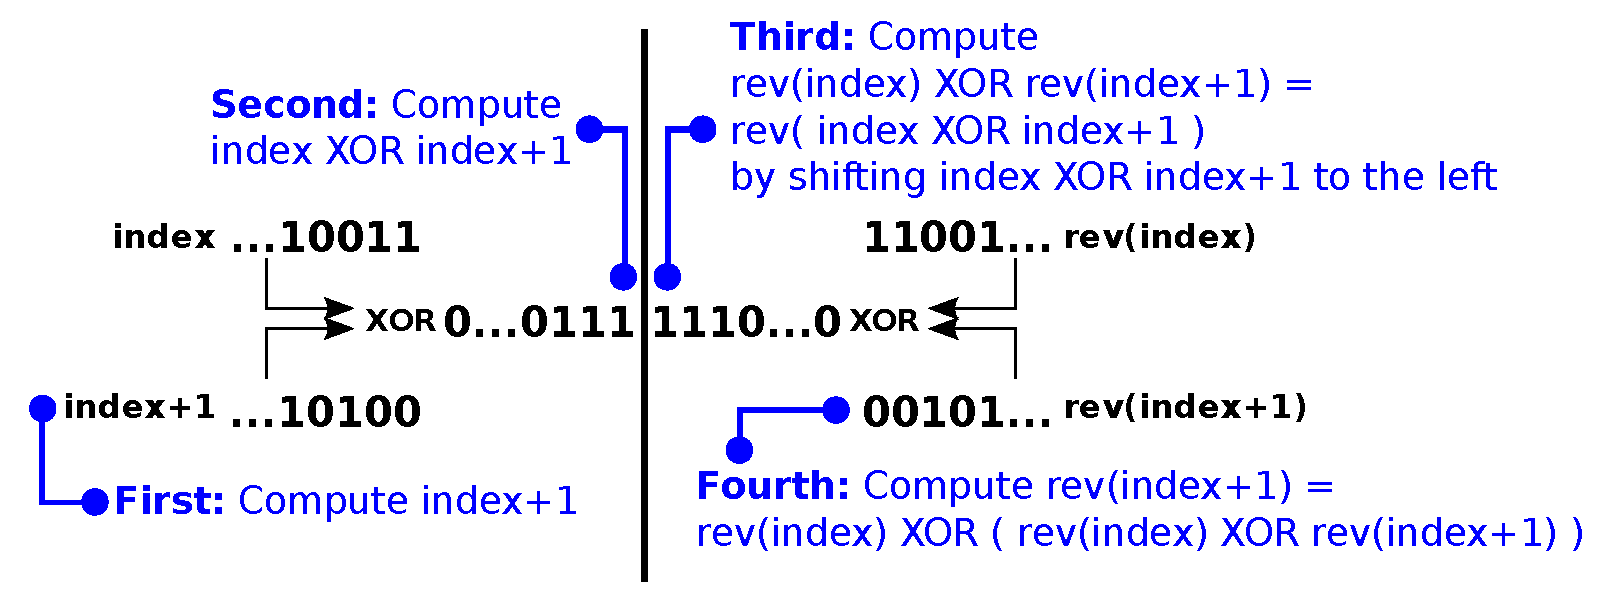
\includegraphics[width=6in]{cartoons/xor.pdf}
\caption{{\bf 归纳异或法实索引现位反转图解。} 由{\tt index}和{\tt rev(index)}开始, 接下来{\tt index}和{\tt rev(index+1)})将被计算。 首先计算{\tt index+1}。 其次,通过异或计算{\tt index}和{\tt index+1}的差异; 位字符串的结果将以{\tt 000\ldots 0111\ldots 1}的形式呈现。再者,因为位的差异为{\tt 000\ldots 0111\ldots 1}形式,可以通过左移CLZ位进行反转。最后,{\tt rev(index+1)}可以按位之间的不同进行反转进行计算获得(异或)。\label{figure:xor}}
\end{figure}

异或法计算下一个索引和下一个索引反转非常高效;然而,即使该计算在瞬时完成,整个算法
的性能也只是中等水平。原因有二:第一个是因为位反转索引并不是连续的在内存中获取。第
二是因为{\tt if}语句,{\bf Listing~\ref{alg:simple-permutation}}也由出现,
它致使循环展开不够高效,因为编译器还不能够预知到在之前的迭代中交换的作用(限制了交
换得并行能力,即使硬件支持)。需要注意的是{\tt index < rev(index)}的次数会在循
环中改变,进而削弱预测的能力。

\paragraph{Unrolling (template-recursive closed form):}

剔除{\tt if (index < rev(index))}的比较是很困难的,因为它需要预先计算进而只
访问结果为真得索引;现有计算的索引模式(if语句为真)和位反转类似。然而,对于固定大小
(如$b = 10$或等价地$n = 1024$)的问题,直接计算那些原本应该进行位互换(位反转变
换)的索引。这将带来两个好处:一是循环之前对索引进行位反转,检测{\tt index < rev
(index)}的情况是否被剔除;二是编译器可以(理论上)重修安排一个连续地位互换操作,进
而改善性能。

这可以通过函数{\tt unrolled\_permutation\_10}实现,也可以通过模板递归
在编译时产生代码。所有{\tt index = z x y}形式的位字符串({\tt z x y}是
 {\tt z}、{\tt x}和{\tt y}串联)其位反转位为{\tt rev(index) = rev(y) rev(x)
  rev(z)}。当{\tt z}和{\tt y}由单个位组成,则其位反转可以忽略:{\tt rev(index) = y
  rev(x) z}。因此,所有可能从位字符串两侧开始(最高位和最低位)并由外向内迭代的处理
相同类型的问题(每一次迭代都调用模板迭代在编译时作展开计算)。部分模板迭代可经分支界面
({\bf Figure~\ref{figure:unrolled}})法排除掉:{\tt index = 1~x~0}形式位字符串
;因而可以舍弃后续的递归。相似地,{\tt index = 0~x~1}形式的为字符串总是小于自身的位
反转{\tt x < rev(x)},因此接下来位互换操作应该对每一个 {\tt x}进行操作。最后,
{\tt 0~x~0}和{\tt 1~x~1}形式的位字符串将小于它们的位反转{\tt x < rev(x)}。这将产
生一个和{\tt index < rev(index)}相类似的情况,但是索引少了两位,所以可以继续使用递归。

所以,该方法的运行时间由循环次数$r(b) = \underbrace{2^{b-2}}_{green} + 
\underbrace{2 \cdot r(b-2)}_{yellow} + \underbrace{0}_{red}$(下表的颜色
对应着{\bf Figure~\ref{figure:unrolled}}中得三种颜色)。令$r(1) = 0$(因为
一位位字符串没有必要进行位互换)和$r(2) = 1$(两位位字符串需要进行一次位互换),
随后得到闭型$r(b) =
2^{\frac{b}{2}} \cdot \left( {(-1)}^b \frac{\sqrt{2}-1}{4} - \frac{1 +
  \sqrt{2}}{4} \right) + 2^{b-1}$。
因此,无论$b$的奇偶性,$r(b) = 2^{b-1} - c \cdot 2^{\frac{b}{2}}$,当$b$为
偶数时$c=\frac{-1}{2}$,当$b$为奇数时$c=\frac{-1}{\sqrt{2}}$。渐进的运行时间
总是由$2^{b-1}$项决定,因此渐进运行时间和$n$ (because $n = 2^b$)成线性关系。

\begin{figure}
\centering
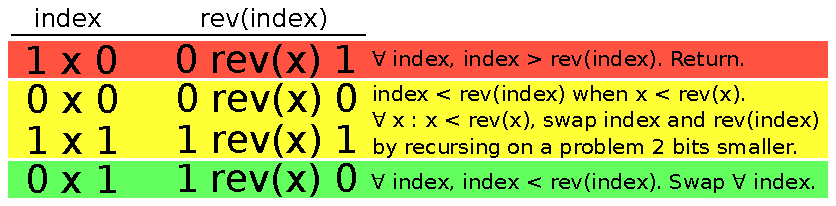
\includegraphics[width=4.5in]{cartoons/unrolled.pdf}
\caption{{\bf unrolled方法实现位反转图解。}
  在编译时发现所有{\tt index < rev(index)}的位字符串,
  {\tt 1~x~0}形式的的位字符串永远不会小于其位反转结果(红色高亮)。{\tt 0~x~1}形式
  位字符串将永远小于其位反转(绿色高亮)。{\tt 0~x~0}和{\tt 1~x~1}形式的位字符串只有
  当{\tt x < rev(x)}的时候才小于其位反转(黄色高亮)。
  \label{figure:unrolled}}
\end{figure}

对于比较小的问题,模板-递归“unrolled”方法非常高效。但是,该方法的一个缺点是当问题
的规模很大时会产生大量的代码,造成编译时间过长,且编译器有可能无法对位互换的顺序做到
优化。事实上,对于缓存而言,可能根本不存在一个高效进行位互换的顺序。因为经位反转的索
引“跳来跳去”。因此,除非编译器能够处理位互换的数学想象(使编译器能够将代码任意切换到
列举出得算法),unrolled方法对于大型问题所表现出的平淡无奇的效率并不能抵消过长的编译
时间。

\paragraph{递归位反转排列组合:}

当位数$b$为偶数时,一个位字符串可以被平分位两个长度为$\frac{b}{2}$的子串:
{\tt index = x~y}。位反转的索引将会是{\tt rev(index)~=~rev(y)~rev(x)}。
该过程可以分为三步:首先,反转最低位({\tt y})得到{\tt x~rev(y)}。其次,位互换
最高位{\tt x}和最低位{\tt rev(y)}得到{\tt rev(y)~x}。最后,重复第一步并反转后几位
({\tt x})得到{\tt rev(y)~rev(x)~=~rev(index)}。

该递归技巧不仅仅对索引位反转计算有用:也对递归方式下整体位反转变换有效。其第一步和第三部
的操作相同:对所有高位的字符串作局部、更小的大小为$\frac{b}{2}$的位反转变换。该递归位反转
将应用于更小的、连续的内存块,从而改善缓存的性能。第二部中,最高位和最低位位字符串的互换对应
着矩阵转置,高位子串对应着矩阵的行,低位子串对应着列(使用{\tt C}样式的行顺序数组)。因为
{\tt x}和{\tt y}有相等的位数,因此位互换对应着一个方阵,可以实现原位操作。众所周知,cache
-oblivious(对任意缓存架构近似最优化)会不断地将问题分解\cite{prokop:cache}。于是位反转
变化可以分解为更小的位反转变化以及方阵转置({\bf Figure~\ref{figure:recursive}})。

\begin{figure}
\centering
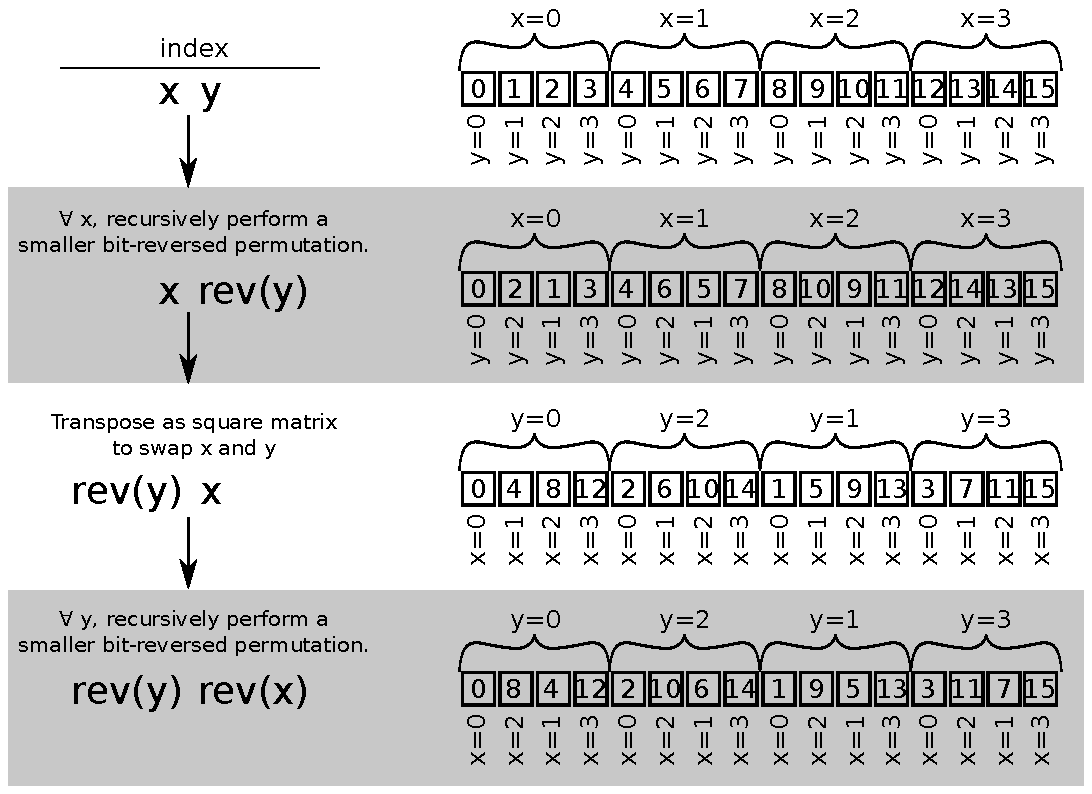
\includegraphics[width=5in]{cartoons/recursive.pdf}
\caption{{\bf 归纳递归位反转组合排列图解。} 一个$b$位位反转组合排列由多个$\frac{b}{2}$
  更小的位反转组合排序、一个矩阵的原地位转置和另外一批$\frac{b}{2}$位的更小位反转组合排列实现。每一步的计算都是在原地覆盖完成,于是有了缓存最佳算法。
  \label{figure:recursive}}
\end{figure}

当$b$为奇数时,执行一次一位奇偶组合排列:由{\tt index = x y z}({\tt z}为一位字符串)
得到{\tt rev(index) = z~rev(y)~rev(x)}。对{\tt z x y}做奇偶变化,在此可以针对
{\tt z}=0和{\tt z}=1做更小的位反转变换。因此,当$b$为奇数时,运行时间将变长,因为奇偶
变化需要一个借用一个大小为$\frac{n}{2}$)的缓冲器实现。

递归方法的运行时间取决于循环$r(b)
= 2 \cdot 2^{\frac{b}{2}} \cdot r(\frac{b}{2}) + 2^b$,次循环解得$r(b) = 2^{b-3} \cdot b \cdot c + 2^b \cdot (b-1)$,$c$为常数。因此$r(b) \in \Theta(2^b \cdot b) = \Theta(n\log(n))$。

尽管在$b \gg 1$时unrolled闭型的缺点,它对小或者中等大小的问题却十分高效,如
$b \leq 14$,对应的$n \leq 16384$);因此,它可以作为递归方法一个理想的基本
案例。递归调用可以使用模板递归。该递归方法会生成一个半递归方法,无论递归的层次
为何,都会调用unrolled实现。这有助于编译器进行优化,因为所有的模板-递归位反转
变换都可以内联的(递归层数较多时,编译器不会内联所有的代码,在{\tt g++}和{\tt
clang}中使用{\tt attribute~(\_\_always\_inline\_\_)}修饰递归位反转组合排
列时,会发现更长的编译时间。)谨记,半递归方法只允许一个$r(b) = 2 \cdot 2^{\frac{b}{2}}
\cdot 2^{\frac{b}{2}} + 2^b$的循环,因为$r(\frac{b}{2})$的循环将被unrolled方法
代替。因此,最终的的运行时间为$2\cdot 2^b + 2^b \in \Theta(2^b) = \Theta(n)$。

递归方法相比COBRA方法的一个优点(至少在$b$为偶数时,$\frac{b}{2}$也是偶数,\ldots
直到基本案例的大小或者达到了递归的极限)是其可以不需要借位于缓冲器而直接原地实现。
因为递归方法将位反转变换问题分解更小的位反转变换问题(各个小问题独立原地执行)和
矩阵转置。其可以通过SIMD并行或使用GPU加速;为了竞争,COBRA的并行需要为每一个并行
复制缓冲器。\newline

所有的渐进运行时间如表所示 {\bf
  Table~\ref{table:theoretical-runtimes}}.

\begin{table}[ht!]
  \centering
  \small
  \scalebox{0.88}{
    \begin{tabular}{c|cccccccc}
      & Stockham & Bitwise & Bytewise & Pair bitwise & COBRA & Unrolled & XOR & Recursive \\
      \hline
      %& \multicolumn{3}{c}{$d$ known at compile time} \\
    {\bf Runtime} & \multirow{2}{*}{$n \log(n)$} & \multirow{2}{*}{$n \log(n)$} & \multirow{2}{*}{$n \log(n)$} & \multirow{2}{*}{$n \log(n)$} & \multirow{2}{*}{$n + \frac{n}{t} \log(\frac{n}{t})$} & \multirow{2}{*}{$n$} & $n$ or & $n$ or \\ 
          (asymptotic) & & & & & & & $n \log(\log(n))$ & $n \log(n)$\\
    \hline
    \end{tabular}
  }
    \caption{{\bf 理论运行时间。} 每一个算法的渐进时间都被给出。时间最短并不意味着在实际使用中也具优势:比如,按位
    和按字节方法皆为$\in \Theta(n \log(n))$,但按字节方法拥有一个更优的运行时间
    常数因为它使用一个查询表,一次反转8位。同样地,按位对、COBRA以及递归方法以更加
    连续、局部的方式使用内存,因此它们更具有高速缓存数据存储性优势。对于COBRA方法,
    $t$是缓冲器的大小。归纳异或法的运行时间可能是$\in \Theta(n)$(计前导零数
    是$\Theta(1)$)或者是 $\Theta(n \log(\log(n)))$(前导零数可由硬件获得,因
    此需要$\in \Theta(\log(\log(n)))$步)。递归方法需要$\in \Theta(n \log(n))$步,当使用限制递归深度的半递归方法时亦可以加速至$\in \Theta(n)$步。
   }
  \label{table:theoretical-runtimes}
\end{table}

\section*{结论}
所有的方法均由{\tt C++11}实现,使用模板递归、{\tt constexpr}变量和函数。所有的运行时
间均经比较,并通过{\tt g++ 5.4.0}和{\tt clang++ 3.8.0}编译实习基准化分析。所有的编译
均由{\tt -Ofast -march=native -mtune=native}优化。
为了避免不同跑分间的指针别名问题,每一个算法以及输入的大小均在不同的{\tt main.cpp}
文件中校准。{\tt g++}的编译时间由{\bf Figure~\ref{fig:g++_compile_times}}
呈现,{\tt clang++}的编译时间由{\bf Figure~\ref{fig:clang++_compile_times}}。
所有的方法均使用{\tt std::complex<double>}类型数组,因为我们的实现快速位反转
变换的最初动机是去评价一个方法是否适合做FFT计算。需要注意的是,各个方法的性能可能
会因为不同的数据类型,如{\tt int}或{\tt float}),而发生变化。

针对原地和非原地的COBRA方法,缓冲器的大小会针对具体的问题进行优化。缓存无视(cache-oblivious
递归方法使用一个COBRA方法中使用的
{\tt log-block-width}参数为$b=20$到$b=26$提供了优化,因此设置为$8$时,

\emph{如}COBRA工作在$2^8 = 256$个元素尺寸的缓冲器,以防止$4096B$大小的
{\tt std::complex<double>}情况。为了防止
缓冲器大小大于问题的大小,所有{\tt log-block-width}将设定小于$2b$。

基准分析问题的大小可以为$n = 2^8$(需要$\approx 4$KB存储空间),也可以$n =
2^{30}$(需要$\approx 16.4$GB存储空间)。所有的结果均经过平均100次的运行,且
每个元素(如$n$次分拣的位反转变换共计消耗的时间)数秒做一次报告。基准分析所用的
CPU的说明如表所示{\bf Table~\ref{table:cpu_spec}}。由{\tt g++}测试的所有运行时间如表
所示{\bf Figure~\ref{fig:g++_runtimes}}。由{\tt clang++}测试的所有运行时间如表
所示{\bf Figure~\ref{fig:clang++_runtimes}}。

为了估量固有的并发特性,半递归方法的并发版本被实现并计算:首先是通过OpenMP的
多核心以及{\tt -fopenmp}编译器操作。OpenMP使用{\tt
\#pragma omp parallel for}来实现递归调用(因为只允许一次递归,所以需要
使用unrolled closed form来实现)。第二个并发修改半递归方法以通过CUDA使用
GPU。该GPU实现允许两个递归并is hard-coded for $b=24$(它需要在数组中存储
经过交换的索引,通过GPU广播)。$b=24$被选中的原因是
它是能够被GPU容纳的最大问题大小,$b$除以4(能被4整除的问题可被展开为两个递归
二无需预先的奇偶组合排列)。CUDA在GPU中做原位转置\cite{harris:cuda},因此
并行递归调用和转置(此法因只需向GPUG写一次数据而具有优势)。OpenMP和GPU都使用
{\tt g++}编译(GPU使用{\tt nvcc}),因为{\tt clang++}缺陷相应的支持。图{\bf
  Figure~\ref{fig:g++_parallel_runtimes}}可与最优的单线程运行做比较。

\begin{table}[ht!]
  \centering
  \begin{tabular}{cccccc} L1d &  L1i &    L2 &      L3 & MAX\_SPEED &   RAM \\
\midrule
 32K &  32K &  256K &  15360K &    3.8Ghz &  65GB \\
\end{tabular}
\caption{ {\bf 用于基准分析的CPU说明。} 显示L1数据缓存大小、
  L1指令缓存大小、L2缓存大小、L3缓存的大小、时钟频率以及内存大小。为了关联我们展示
  的基准分析,其中$32$K内存可容纳一个拥有$n=2^{11}$个元素的{\tt std::complex<double>}
  类型数组,$256$K可容纳一个拥有$n=2^{14}$个元素的{\tt std::complex<double>}
  类型数组, $15360$K可以容纳$n=2^{20}$个元素。$65$GB可以容纳$n=2^{31}$个
  元素。
  \label{table:cpu_spec}
}
\end{table}

\begin{figure}[ht!]
\centering
\begin{tabular}{cc}
  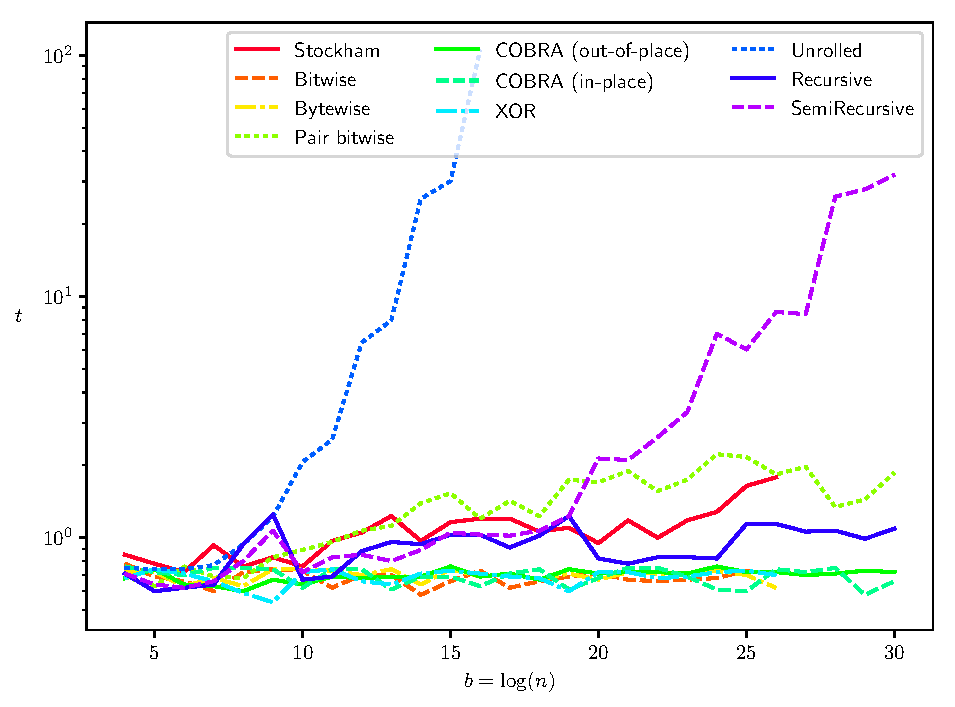
\includegraphics[width=4.5in]{results/g++_compile_times.pdf}
\end{tabular}
\caption{{\bf {\tt g++}的编译时间}。 每一种方法,其各规模的位反转排列组合的编译时间
   如图所示。$t$轴按对数比例缩放。每种方法的运行时间在图\ref{fig:g++_runtimes}中描述。
   $b>16$时,UnrolledShuffle不再计算,因为无论是可执行性还是编译时间都远远超出了我们的
   接受范围。
  \label{fig:g++_compile_times} 
}
\end{figure}


\begin{figure}[ht!]
\centering
\begin{tabular}{cc}
  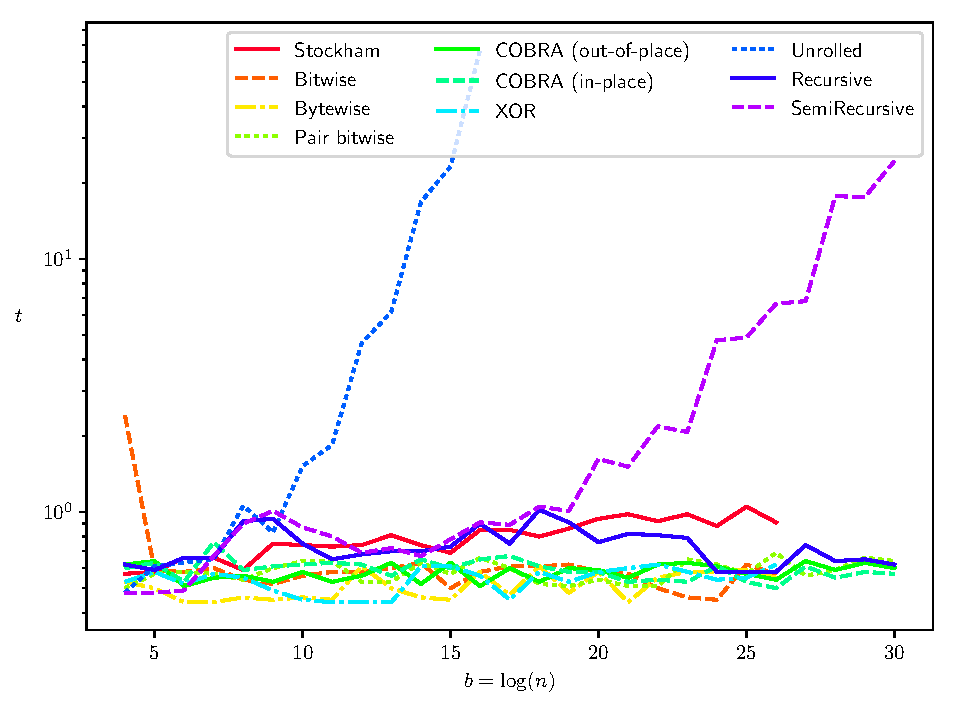
\includegraphics[width=4.5in]{results/clang++_compile_times.pdf}
\end{tabular}
\caption{{\bf {\tt clang++}的编译时间}。           每一种方法,其各规模的位反转排列组合的位反转排列组合的编译时间
   如图所示。$t$轴按对数比例缩放。每种方法的运行时间在图\ref{fig:clang++_runtimes}中描述。
   $b>16$时,UnrolledShuffle不再计算,因为无论是可执行性还是编译时间都远远超出了我们的
   接受范围。
  \label{fig:clang++_compile_times} 
}
\end{figure}

\begin{figure}[ht!]
\centering
\begin{tabular}{cc}
  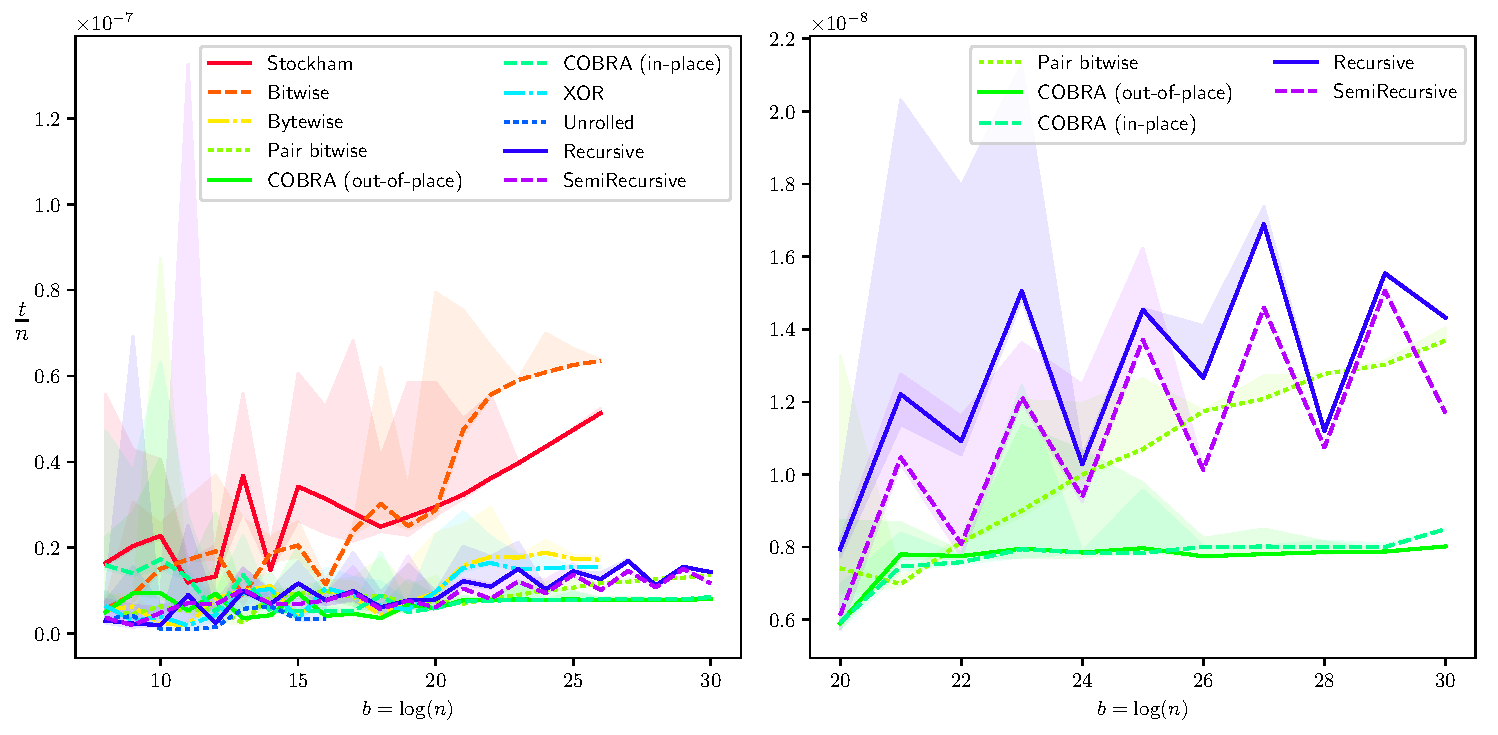
\includegraphics[width=6in]{results/g++_run_times.pdf}
\end{tabular}
\caption{{\bf {\tt g++}下,每个元素的运行时间}. 
  每一种方法,完成其各规模的位反转排列组合的位反转排列组合。每一种重复运行100次
  (按秒计)被测试,每一元素的平均运行时间(\emph{i.e.},消耗时间除以$n = 2^b$)
  如图所示。阴影区域描述了100次下96\% 的情况(\emph{i.e.},前2\%以及后2\%被排除)。
  左侧图片显示了全部方法从$b=4$至$b=28$的情况,右侧图片只显示在大规模问题$b=20$到
  $b=28$情况下的最高性能。为了节约时间,从$b>26$开始,排除那些注定在大规模问题上低效的方法是很有意义的,如:Stockham、按位、按字节以及异或。
  由于内存限制,非原地COBRA方法不能做$b=28$的运行。
  \label{fig:g++_runtimes}  
}
\end{figure}

\begin{figure}[ht!]
\centering
\begin{tabular}{cc}
  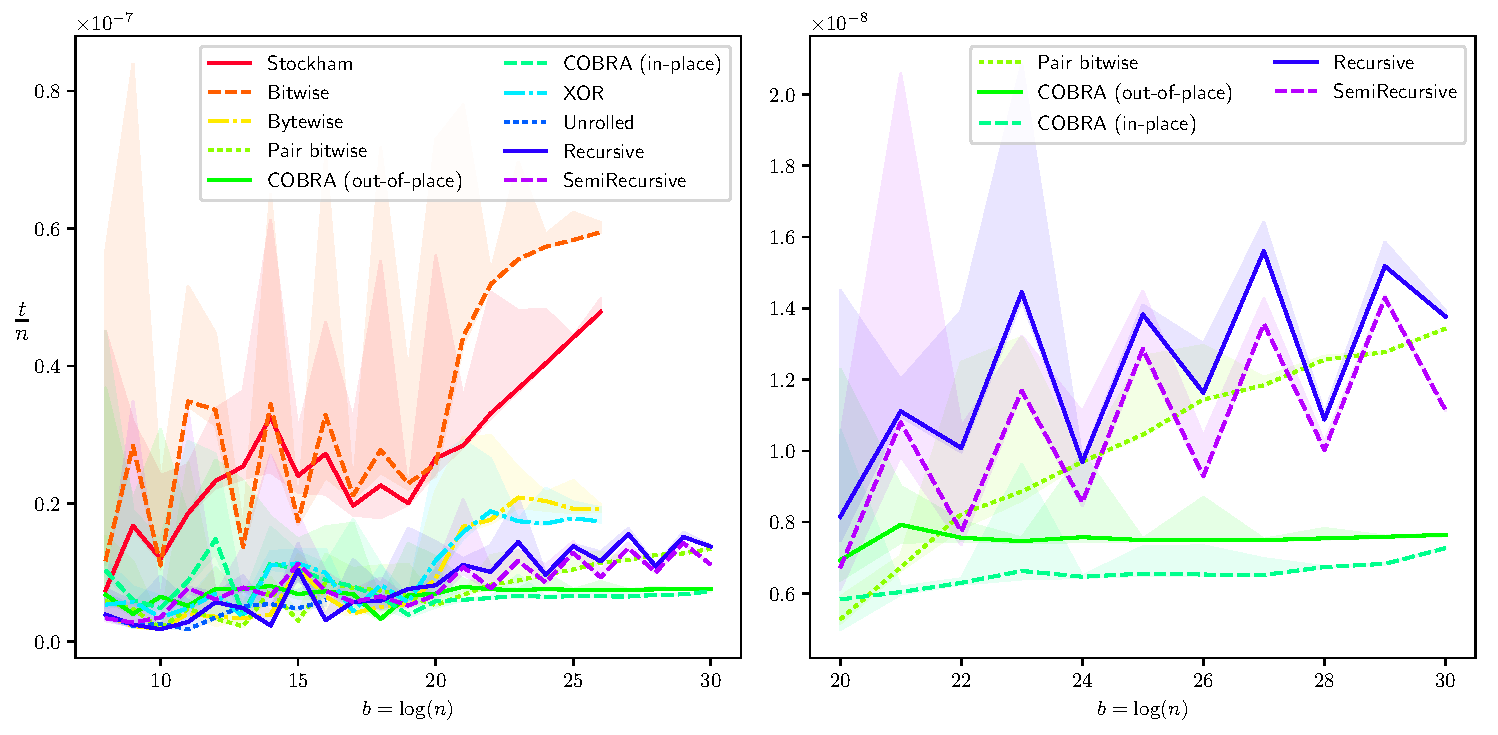
\includegraphics[width=6in]{results/clang++_run_times.pdf}
\end{tabular}
\caption{{\bf {\tt clang++}下每个元素的运行时间}. 每一种方法,完成其各规模的位反转排列组合的位反转排列组合。每一种重复运行100次
  (按秒计)被测试,每一元素的平均运行时间(\emph{i.e.},消耗时间除以$n = 2^b$)
  如图所示。阴影区域描述了100次下96\% 的情况(\emph{i.e.},前2\%以及后2\%被排除)。
  左侧图片显示了全部方法从$b=4$至$b=28$的情况,右侧图片只显示在大规模问题$b=20$到
  $b=28$情况下的最高性能。为了节约时间,从$b>26$开始,排除那些注定在大规模问题上低效的方法是很有意义的,如:Stockham、按位、按字节以及异或。
  由于内存限制,非原地COBRA方法不能做$b=28$的运行。
  \label{fig:clang++_runtimes}  
}
\end{figure}

\begin{figure}[ht!]
\centering
\begin{tabular}{cc}
  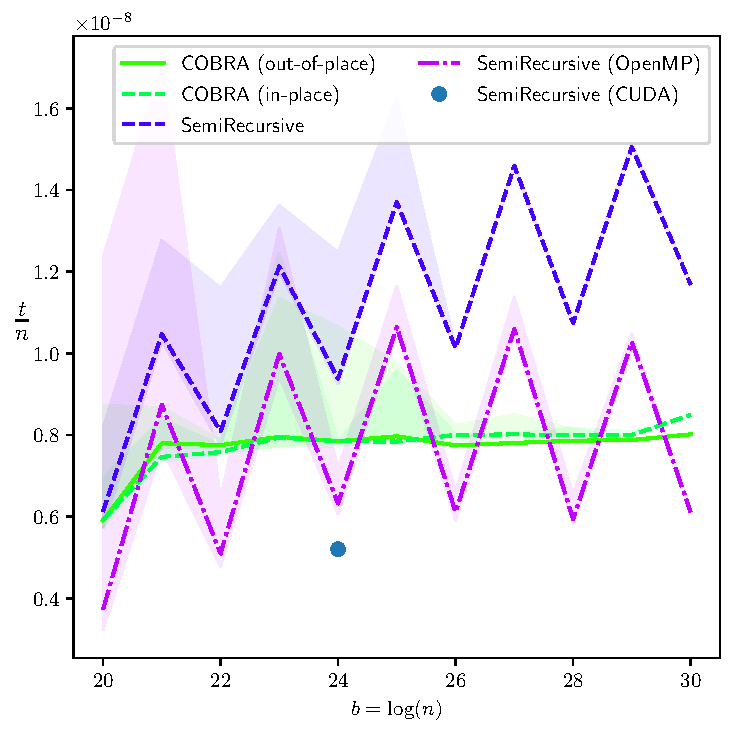
\includegraphics[width=6in]{results/open_mp_performance.pdf}
\end{tabular}
\caption{{\bf 并行的性能}. 基准分析从{\bf Figure~\ref{fig:g++_runtimes}}
   开始被反复提及,包含了并行半递归方法。由于半递归法的固有并行性,OpenMP可以轻松的获得更快的速度。
   同样地,GPU上的广播操作(通过CUDA)可以获得更好的并发性。

  \label{fig:g++_parallel_runtimes}
}
\end{figure}


\section*{讨论}

经{\tt g++}和{\tt clang++}验证,Stockham和朴素按位shuffling方法性能相当,
都属于最不高效的行列。Stockham方法是一种非原地方法(因而增加缓存负荷)而且比
按位shuffle执行更多的交换操作;然而,Stockham方法以奇数项和偶数项的方式读取
数据,相较于按位法在每次循环中读取数据{\tt rev(i)},该方式读取的数据大体上可
以地认为更加的连续。

按字节查找表方法和异或方法拥有相似的表现。两种方法较Stockham和按位方法具有较
大的性能提升,且二者均获得了更快的位反转,然二者都没有以相对连续的方式读取内存;
因此,二者的缓存利用能力较差。被提倡的异或法或许依旧在内存稀缺的场景下被使用
(\emph{比如},嵌入式系统,因此在不存储或读取大小为$256$B表的情况下,异或法取
得了与查表法相似的性能表现。

对于比较小的问题,unrolled方法获得可观的优化性能,L1缓存可以容纳整个数组并且
循环、位反转或分支语句没有遇到瓶颈;然而,较大的问题却不同于此(数组不能全部置
于L1和L2缓存),甚至unrolled方法的编译时间也变得糟糕(当$b=16$,{\tt g++}
和{\tt clang++}的编译时间约为100秒)。

时刻考虑缓存的方法在大规模问题的处理上更显得优异:这包括了按位对方法、COBRA方法
(原地和非原地)、递归
方法以及其半递归变种。特别地,递归和半递归方法在偶数位大小的问题上具有优势,因
为奇偶组合排列的预操作可以被省略(大型问题的运行时间呈锯齿状)。半递归方法相较
于递归方法,获得微小的性能提升,却也付出了相应的代价($b=28$时,{\tt g++}和
{\tt clang++}的编译时间在10到13秒之间)。对于小型问题,非原地COBRA方法的性
能弱于原地变体,皆因为两次重度使用高速缓存,而原地方法却通过缓冲器交换;因此原
地方法必须向缓冲器拷贝数据,在数据和缓冲之间接交换,将改变的数据从缓冲器中拷
贝入数组。

按位对方法执行更多的交换操作,但是更好的内存地址读取性且不需要使用一个结果
缓冲器(而这却是非原地算法需要的,如Stockham)。按位对、COBRA法、递归法以及半
递归法对于大型问题的性能可等量齐观;非原地COBRA法在大型问题上稍具优势,然而最佳
状态并不稳定,矩阵缓冲器尺寸需针对CPU预习做出优化。高一级的高速缓存中每位元素的
运行时间都会些许增加,尤其是L3高速缓存中$b=18$
的原地方法和$b=17$的非原地方法。

不同于COBRA方法通过矩阵缓冲器提升性能,递归和半递归法是“天然”的高速缓存高效法并
且无需缓冲器;因此,它们非常适合做并行计算。如{\bf Figure~\ref{fig:g++_parallel_runtimes}}显示,通过OpenMP增加粗粒度并行计算或者通过GPU增加细粒度
并行计算可以显著提升性能。递归无需从其他元素获取信息,因而呈现完美的并发性(包括
当下每个核心包含独立的L1高速缓存的情况)。这样“与生俱来”的并发优势可以在未来优化的
GPU代码发挥作用。

在Figure~\ref{fig:g++_parallel_runtimes}中,当$b=24$时,最快的非并行方法
每一个元素需要$8 \times{10}^{-9}$,总计约$0.13$秒。相比较,半递归OpenMP变体
需要约$0.1$秒,其GPU变体只需$0.08$秒。文献中有一观点:{\tt numpy} FFT(使用
{\tt FFTPACK}包)对于同体量的问题却需要近2秒。朴素按位法需要约1秒,其中包括50\%
的FFT运行时间花费在位反转组合排列上,意味着通过使用更快的位反转组合排列去提升速度
并不是无足轻重的;虽然蝴蝶操作代码对复数进行更加复杂的组合排列,但是其以一种完全内
存连续的方式工作,让位反转组合排列的重要性更加凸显。此外,在GPU使用半递归法实现
完整的FFT,不仅可以从小规模的并行FFT蝴蝶操作中受益,而且可以大幅度地减少位反转排
列组合的运行时间,进而避免数据往复GPU的消耗。

除递归方法的并发性外,它们可以在不寻求特定的高速缓存结构(COBRA法受高速缓存架构
影响)的情况下,获取高性能。特别地,递归法是一种缓存无视方法。当转置时\cite{prokop:cache},
它可在不获取快速缓存架构的情况下保证相当连续的内存读取。同递归法类似,半递归策略
亦不使用经大小优化的缓冲器;然,半递归法不是一种缓存无视方法,因为即使经过分割的
大规模问题,其子位反转排列组合问题的大小亦不适于高速缓存。递归问题不仅对往后研
究并行计算效益的工作显得有趣,其不知架构即可提高性能的特点亦值得后人对最佳缓存无
视位反转排列组合算法驻足。



\section*{Availability}
本文所有的{\tt C++}源代码、初步的GPU递归算法实现、基准分析脚本以及本文的\LaTeX\ 
源码都可以自由获取(创作公用许可)。
请访问:\url{https://bitbucket.org/orserang/bit-reversal-methods}.\newline

\section*{鸣谢}

我们感谢Thimo Wellner和Guy Liang对本文提供的帮助\newline 

\noindent 本文的撰写将作为柏林自由大学2016-2017年度冬季学期科学计算课程的一部分。该课程
由Oliver Serang执教,本文由多名学生提供母语翻译。(德语、汉语、土耳其语以及西班牙语
翻译于repository链接中可见)。

\section*{作者贡献}
该文章的新算法和独特的{\tt C++11}实现由O.S.发明并指导完成。引言由X.W编写。方法部分
和运行时间的分析由B.A.、D.W.与X.W. 完成。OpenMP实现由O.S.完成。GPU部分由B.A和D.W实现。
基准分析、作图以及结论部分由C.K.完成。讨论部分由C.K.和X.W.完成。测试和优化由B.A与D.W实现。
最终的基准分析由C.K.、L.I.、T.C.、与O.S.\newline

% at end of this section:
\noindent 除了最后作者(O.S.和T.C.),其他作者顺序由全体投票产生。

% bibliography:
\bibliographystyle{unsrt}
\bibliography{refs.bib}

\clearpage\end{CJK*}
\end{document}

